% A CONSORT-style flowchart of a randomized controlled trial
% using the PGF/TikZ package
% Author  : Morten Vejs Willert (July 2010)
% License : Creative Commons attribution license
\documentclass{article}
\usepackage[latin1]{inputenc}
\usepackage{tikz}
\usetikzlibrary{shapes,arrows}
\usepackage{caption}
\newcommand*{\h}{\hspace{5pt}}% for indentation
\newcommand*{\hh}{\h\h}% double indentation
\begin{document}
\begin{center}
  \captionof{figure}{Flowchart of participants' progress through
    the phases of the trial}
  % setting the typeface to sans serif and the font size to small
  % the scope local to the environment
  \sffamily
  \footnotesize
  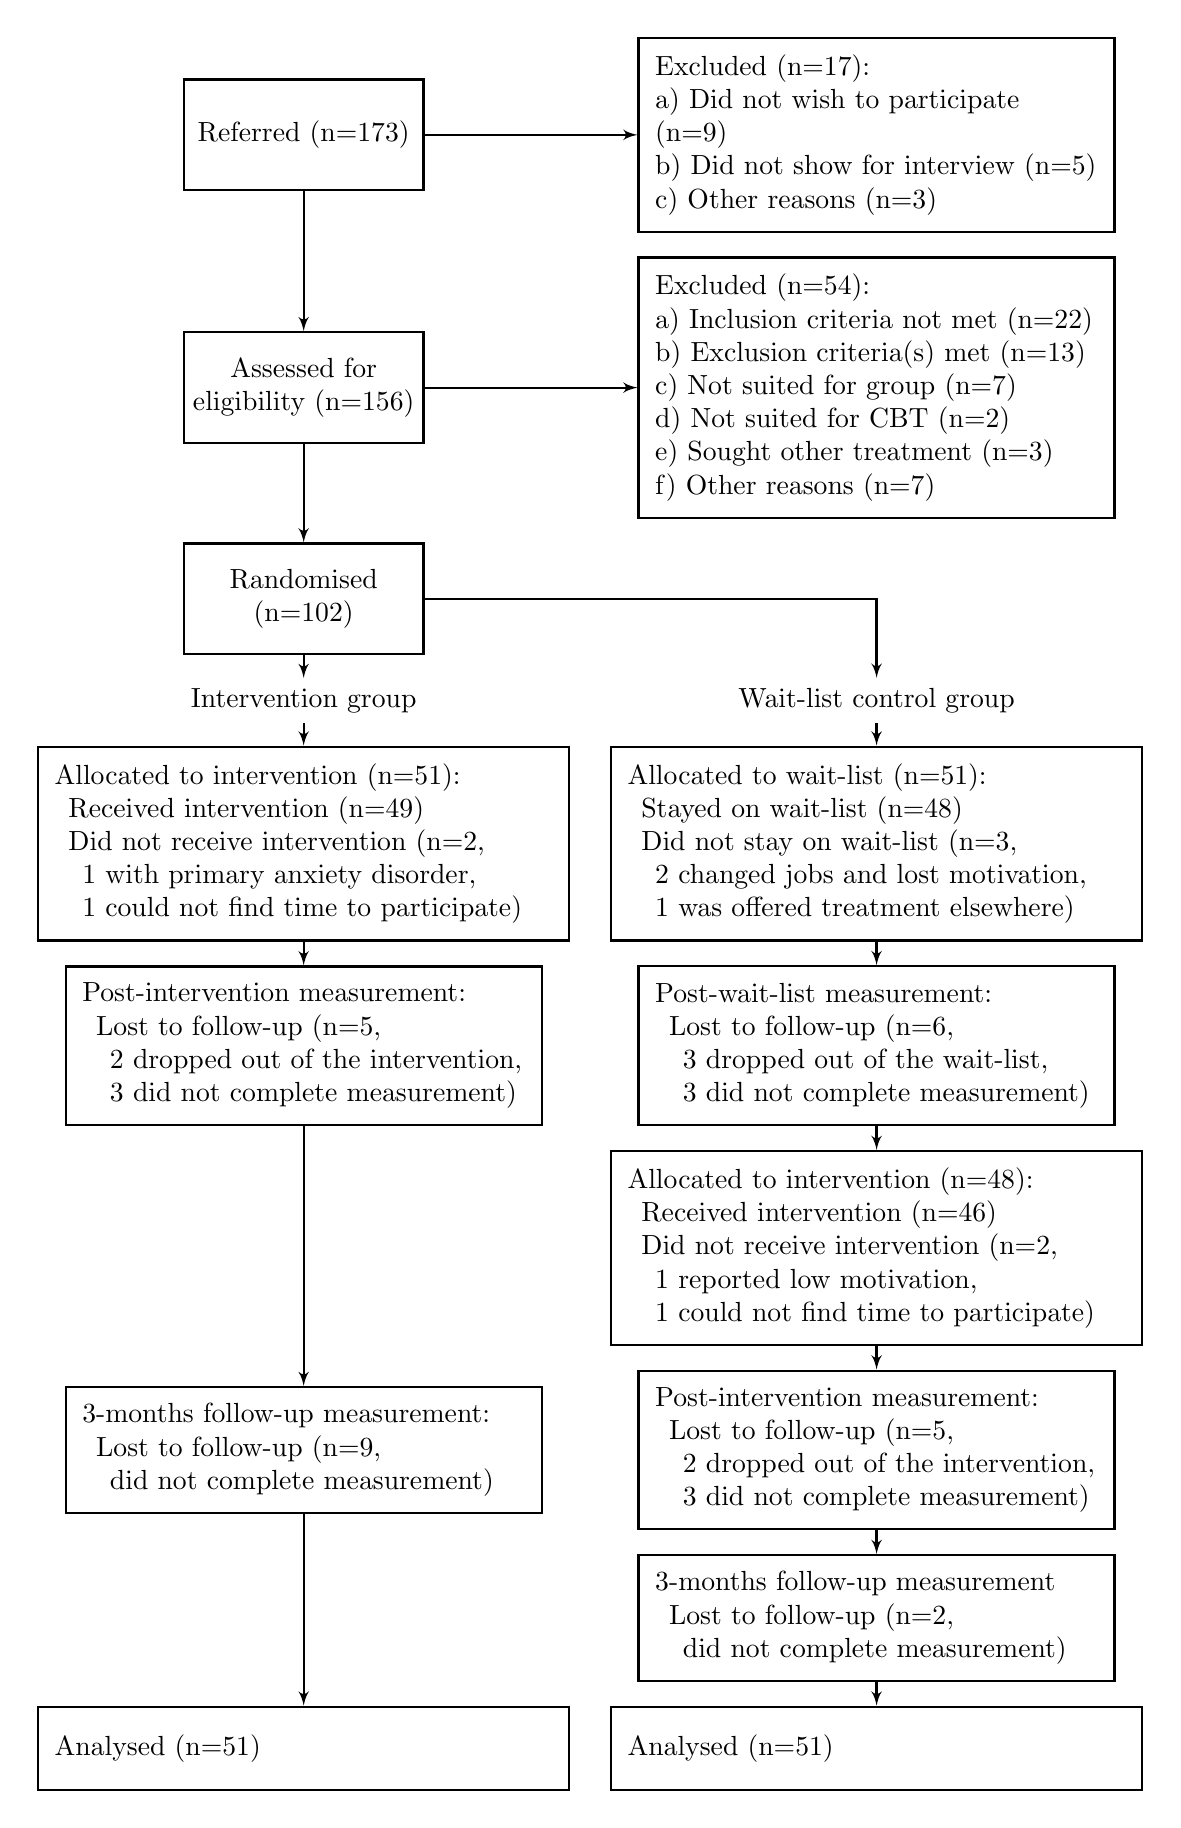
\begin{tikzpicture}[auto,
    %decision/.style={diamond, draw=black, thick, fill=white,
    %text width=8em, text badly centered,
    %inner sep=1pt, font=\sffamily\small},
    block_center/.style ={rectangle, draw=black, thick, fill=white,
      text width=8em, text centered,
      minimum height=4em},
    block_left/.style ={rectangle, draw=black, thick, fill=white,
      text width=16em, text ragged, minimum height=4em, inner sep=6pt},
    block_noborder/.style ={rectangle, draw=none, thick, fill=none,
      text width=18em, text centered, minimum height=1em},
    block_assign/.style ={rectangle, draw=black, thick, fill=white,
      text width=18em, text ragged, minimum height=3em, inner sep=6pt},
    block_lost/.style ={rectangle, draw=black, thick, fill=white,
      text width=16em, text ragged, minimum height=3em, inner sep=6pt},
      line/.style ={draw, thick, -latex', shorten >=0pt}]
    % outlining the flowchart using the PGF/TikZ matrix funtion
    \matrix [column sep=5mm,row sep=3mm] {
      % enrollment - row 1
      \node [block_center] (referred) {Referred (n=173)};
      & \node [block_left] (excluded1) {Excluded (n=17): \\
        a) Did not wish to participate (n=9) \\
        b) Did not show for interview (n=5) \\
        c) Other reasons (n=3)}; \\
      % enrollment - row 2
      \node [block_center] (assessment) {Assessed for eligibility (n=156)}; 
      & \node [block_left] (excluded2) {Excluded (n=54): \\
        a) Inclusion criteria not met (n=22) \\
        b) Exclusion criteria(s) met (n=13) \\
        c) Not suited for group (n=7) \\
        d) Not suited for CBT (n=2) \\
        e) Sought other treatment (n=3) \\
        f) Other reasons (n=7)}; \\
      % enrollment - row 3
      \node [block_center] (random) {Randomised (n=102)}; 
      & \\
      % follow-up - row 4
      \node [block_noborder] (i) {Intervention group}; 
      & \node [block_noborder] (wlc) {Wait-list control group}; \\
      % follow-up - row 5
      \node [block_assign] (i_T0) {Allocated to intervention (n=51): \\
      \h Received intervention (n=49) \\
      \h Did not receive intervention (n=2, \\
      \hh 1 with primary anxiety disorder, \\
      \hh 1 could not find time to participate)}; 
	  & \node [block_assign] (wlc_T0) {Allocated to wait-list (n=51): \\
      \h Stayed on wait-list (n=48) \\
      \h Did not stay on wait-list (n=3, \\
      \hh 2 changed jobs and lost motivation, \\
      \hh 1 was offered treatment elsewhere)}; \\
      % follow-up - row 6
      \node [block_lost] (i_T3) {Post-intervention measurement: \\
      \h Lost to follow-up (n=5, \\
      \hh 2 dropped out of the intervention, \\
      \hh 3 did not complete measurement)}; 
	  & \node [block_lost] (wlc_T3) {Post-wait-list measurement: \\
      \h Lost to follow-up (n=6, \\
      \hh 3 dropped out of the wait-list, \\
      \hh 3 did not complete measurement)}; \\
      % follow-up - row 7
      % empty first column for intervention group 
      & \node [block_assign] (wlc_T36) {Allocated to intervention (n=48): \\
      \h Received intervention (n=46) \\
      \h Did not receive intervention (n=2, \\
      \hh 1 reported low motivation, \\
      \hh 1 could not find time to participate)}; \\
      % follow-up - row 8
      \node [block_lost] (i_T6) {3-months follow-up measurement: \\
      \h Lost to follow-up (n=9, \\
      \hh did not complete measurement)}; 
      & \node [block_lost] (wlc_T6) {Post-intervention measurement: \\
      \h Lost to follow-up (n=5, \\
      \hh 2 dropped out of the intervention, \\
      \hh 3 did not complete measurement)}; \\
      % follow-up - row 9
      % empty first column for intervention group 
      & \node [block_lost] (wlc_T9) {3-months follow-up measurement \\
      \h Lost to follow-up (n=2, \\
      \hh did not complete measurement)}; \\
      % analysis - row 10
      \node [block_assign] (i_ana) {Analysed (n=51)}; 
      & \node [block_assign] (wlc_ana) {Analysed (n=51)}; \\
    };% end matrix
    % connecting nodes with paths
    \begin{scope}[every path/.style=line]
      % paths for enrollemnt rows
      \path (referred)   -- (excluded1);
      \path (referred)   -- (assessment);
      \path (assessment) -- (excluded2);
      \path (assessment) -- (random);
      \path (random)     -- (i);
      \path (random)     -| (wlc);
      % paths for i-group follow-up rows
      \path (i)          -- (i_T0);
      \path (i_T0)       -- (i_T3);
      \path (i_T3)       -- (i_T6);
      \path (i_T6)       -- (i_ana);
      % paths for wlc-group follow-up rows
      \path (wlc)        -- (wlc_T0);
      \path (wlc_T0)     -- (wlc_T3);
      \path (wlc_T3)     -- (wlc_T36);
      \path (wlc_T36)    -- (wlc_T6);
      \path (wlc_T6)     -- (wlc_T9);
      \path (wlc_T9)     -- (wlc_ana);
    \end{scope}
  \end{tikzpicture}
\end{center}
\end{document}